%Main Document
\documentclass[a4paper, 11pt, oneside]{AuProjectHandin} % loads the layout.
\usepackage{AuPreamble} % loads the Preample
%\usepackage{hyperref}
%configurationfile
\pagestyle{AuHandin}

\title{E18 E6BAC-01}

%author is not used in generating the content for the tile page so is not needed. use the group members function instead.
%\author{Tonni Follmann}

%Vejlederens navn
\SetVejleder{Torben Gregersen}
%Skole/Universitetets navn
\SetUniversity{Aarhus University}
%Projektnavn
\SetProject{Designing Multichannel Audio- and Video-Playback System: Showman}
%Produktnavn
\SetProductname{Preparation for Bachelor Project}
%Gruppe Nummer
%\SetGroupNumber{5}
%Add the names of all the members in the group, can handle 1 to 8 members, names are added one per set of [], that means if only 1 person should be the author of this document, only one set of brackets [] are needed.
\GroupMemberNames[Minik Nathanielsen Olsen]{}
%add student numbers of the students, must have the exact same order as the names listed above.
\GroupMemberStudentNo[201600341]{} % loads configuration file
\begin{document} % begins the document
%titlepage
\begin{titlingpage}
	\center


	% Display product name and document title
	\HUGE\ShowProductName \\
	\huge\thetitle

	\vspace{10 mm}
	% Display group number and project term.
	\Large\ShowProject

	%\Large Gruppe \ShowGroupNumber

	\vspace{10 mm}
	% Show counselor on from page
	%\normalsize Counselor: \ShowVejleder
	\vspace{10 mm}

	%Generate a table of group members as authors of the document.
	Group members:

	\PrintGroupMembers


\end{titlingpage}
 % generates titlepage

\frontmatter
%\input{versioning}
% Front matter is the section where table of contents, thank notes, abstract etc should be placed.
\tableofcontents
%\input{glossary}
%generate  table of content etc here (filler stuff)
\mainmatter
%main matter is the true content of the report. include your content files here
%using \input{filename}. No preamble etc should be in the files that are being included.
% \begin{document} etc should not be included in the files either.
\chapter{Project Description}
The following text is the project description pulled from the project catalog. \newline

Development of multi-channel audio/video playback system for touring artists. This project will
integrate both hardware- and software-design with emphasis on hardware design.
Approx. 70-80 percent of modern Danish and international touring artists utilize audio backing tracks
(prerecorded material played back on some chosen device) and video content projected on large
screens as part of their performance. \newline

However, there are a multitude of options ranging from iPod-playback to complex, customized
systems operated by technical personnel. \\
Common for these systems is instability, making artists to purchase redundant backup-systems in
order to deliver their audience a flawless and uninterrupted performance. \newline

In a typical scenario, at least one laptop – often several laptops – with various audio- and/or videointerfaces, handles and runs the audio backing track and video-content in sync. \newline

This project will integrate both audio- and video-handling in a single 19” rack-mounted device and
provide the user with a user-friendly GUI (Graphical User Interface) while complying with
international standards for audio and video and electronic devices. \newline

For design and implementation of the device, a research is needed in: \\
- Circuit/hardware design \\
- D/A audio converters \\
- Standardized audio input/output formats \\
- Audio file formats \\
- Standardized video input/output formats \\
- Video file formats \\
- Time codes for synchronization \\
- User feedback for feasible GUI design \newline

This project is already in the early stages of development as part of an apprenticeship in
entrepreneurship (iværksætterpraktik) at Navitas Science and Innovation. \\
Current status on project: \\
- Requirements specification finished \\
- FURPS finished \\
- Market research ongoing \newline

The project is requesting confidentiality as the device is in development intended for market release to
prosumers in the music industry, thus an eventual project partner must sign a non-disclosure
agreement. \newline

Project partner profile: Electronic Engineering student or Information and Communication
Technology student.
\chapter{Requirement Specification}
(Udkast til) kravspecifikation
\chapter{Project Plan}
This section is an excerpt of the project plan. The project plan features descriptions of which experiments, technologies etc. to conduct and investigate during the Bachelor's Project. \newline

This section contains how the project work will be structured, which methods to be used, etc. \newline

The Bachelor’s Project (Thesis or Final Project) is an extensive project dealing with a realistic engineering assignment. The bachelor project should document the students’ ability to work independently to apply engineering methods and theories in solving professional problems and development issues in a specific field. The project constitutes the conclusion of the programme and is placed in the last semester. \newline

The Bachelor's Project workload is 20 ECTS points. 1 ECTS translates to 27 hours of workload, totaling 540 hours of workload for the Bachelor's Project. Assuming 18 weeks of Bachelor's Project work, total workload/week is 30 hours/week. \newline

During the project period, 2 elective courses with 10 ECTS points in total to fulfil the goal of 30 ECTS workload each semester. Assuming 18 weeks of lectures and assignments, total workload/week is ~16-17 hours/week. \newline

Total workload is expected to be ~45-50 hours/week during the semester. To keep track of the project, weekly meetings with supervisor is essential along with project management tools: The ASE-model, SCRUM and Redmine. \newline

\subsection{ASE-model}


\subsection{SCRUM}


\subsection{Redmine}


\subsection{Supervisor Meetings}


\subsection{Timetable}
%\textbf{Objective} \\
%The objective of the Bachelor’s Project is that students be able to plan and conduct an engineering project in as realistic a form as the study environment allows, preferably in cooperation with companies. \\

%\textbf{Learning Objectives} \\
%Upon completion of the Bachelor’s Project, the student should be able to: \\

%- Apply scientific research results and technological knowledge for solving  technical problems, \\
%- Develop new solutions, \\
%- Acquire and evaluate new knowledge within relevant engineering fields, \\
%- Systematically apply engineering knowledge, theories and methods \\
%- Plan and complete a project in a group in cooperation with internal and external partners \\
%- Present results of a project in writing and orally by means of relevant communication tools, to professionals as well as customers, \\
%- Present results of a project orally and with means of various audio or visual communication tools, \\
%- Integrate social, economic, environmental and work environmental consequences in the solution model \newline

%Learning objectives in relation to the specific subject and with reference to above, including their weight, is specified in the Assignment Formulation. \newline

%\textbf{Main Content} \\
%The Bachelor’s Project should comprise the planning and documentation of solutions for a realistic engineering project or defined parts and comprise independent experimental, empirical and/or theoretical discussions and computations. \\

%\subsection{Project Plan}
%Project management tools are needed for the project to keep focus. Aarhus School of Engineering development model 
\chapter{Project Research}
This section investigates similar projects and products. Market analysis was conducted in the fall of 2018 to create an overview of the market. 70+ key figures from the Danish and international music business - musicians, recording producers, touring personnel, etc. - were interviewed for an investigation of their consumption patterns, gear run downs, their requests for useful features and the pitfalls of their gear. \newline

The most experienced users are the so-called \textit{backline technicians} (or backliners) that travel/tour with a touring artist or band to set up, tear down and maintain the artists' instruments and gear. In addition to setting up and tearing down the gear, the backline technician often operates electronics that run parts of the show such as backing tracks on some chosen device, MIDI changes, tune guitars/basses during the perfomance - In general to assist in making the artist's performance to run smoothly without unnecessay interruptions. \newline

The most experienced backliners actively explore and research new technologies and products in between tours and/or during their spare time. Some even modify hardware and software to suit their clients' needs. And some backliners - usually on tours with larger production budgets - even design customized systems. \newline

Indeed, touring personnel - whether they are backliners, sound engineers, lighting engineers, etc. - are passionate about their job and they continually explore solutions to make a performance to run even more smoothly. \newline

The common denominator in the interviews is the critical need for stability. Some of the technologies outlined later in this section have trade-offs: Some sacrifice user-friendly GUIs to ensure stability, some trade-offs are loss in audio quality to ensure stability and user-friendly GUI and vise versa. \newline

As several of the available technologies heavily rely on laptops and home-made systems during performances, the incentive to produce Showman is to remove laptops from the perfomance scenario to avoid hiccups during a show. \newline

Following subsections briefly introduce the most popular tehcnoloqies used currently by touring artists and their personnel with a list of their pros and cons. This chapter concludes with an introduction of Showman's desired features. \\

\subsection{Similar Projects}
This subsection investigates similar projects from Scandinavia. \\

\subsubsection{Interactive Performance System}
Mircea Gabriel Eftemie, Medialogy-alumni from Aalborg University developed a system called '\textbf{Interactive Performance System}', a visual system for concert performances: https://videnskab.dk/kultur-samfund/heavy-metal-pa-universitetet. The project was developed using Open Source technology as his Bachelor's Project with fellow students Thomas Wisbech, Lasse Wingreen and Brenly Bernard. \newline

The purpose of the system was to display theatrical and visual elements during performance without the aid of technical personnel to enhance the performance experience for the audience. The system combined two inputs: A static and dynamic input. The static inputs were prepared beforehand. The static inputs were controlled by an input during the performance partly from a webcam that filmed the audience and the artists and partly from a microphone that recorded and transmitted the audio on stage. \newline

Mircea played guitar in now-defunct Mnemic that utilized the Interactive Performance System. The project was put to rest after Mnemic's dissolution and the project status remains unclear. \\

\subsubsection{The Dark Player}
Members of Swedish band Darkane developed a system for backing track playback device called '\textbf{The Dark Player}' after expressing dissatifaction with current products available. I am in the process of tracking down the members to investigate their system further. \\

\subsection{Similar Products}
Digital Audio Workstations are the hub for 99 percent of all modern musicians and producers. (Source: https://ask.audio/articles/the-top-11-most-popular-daws-you-voted-for) \newline

Products similar to Showman exist in many forms: From simple iPods to complex systems, artists can pick and choose any system available in several configurations depending on financial status. However, some proves to be too unreliant, unstable or reliant on other pieces of hardware to function as intended. The subsubsections below outlines the most widely used products. This subsection conludes with Showman's intended features. \\

\subsubsection{Cymatic Audio LP-16}
The LP-16 (http://cymaticaudio.com/lp-16-productpage/) is a multi-track player for live perfomances that spares the user of using laptop and computer audio interface in a live environment. Its primary use is backing tracks, but its other features include virtual sound checks, triggering synthesizers or samplers, drigin light shows and controlling devices. \\

- Direct from USB hard drive multi-track playback: 16 tracks at 24-bit, 44.1/48 kHz
- Creation and editing of setting and playlist offline with software uTool
- 16 \textit{unbalanced} analog 1/4'' tip-sleeve outputs
- Mac OS-X and Windows PC compatible
- 249 EUR at thomann.de

\begin{figure}[H]
\centering
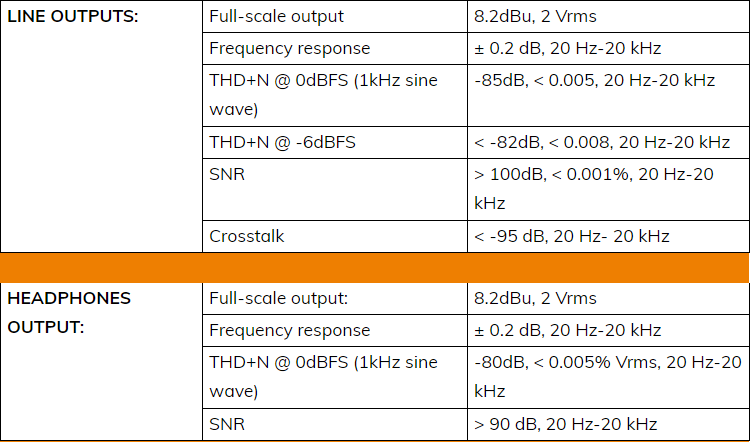
\includegraphics[scale=0.7]{./pictures/lp16.png}
\caption{Selected specifications of Cymatic Audio LP-16 Live Player}
\label{fig:lp16.png}
\end{figure}

Minimum requirements for connection to mixing board: \\

- Up 16 x 1/4'' tip-sleeve jack-cables: 14.90 EUR for the sssnake MPP8030 at thomann.de \\
- Up to 16 x line drivers: 2 x 103 EUR (Behringer DI800 Ultra-DI PRo v2 from thomann.de): 206 EUR \\
- USB hard drive: SanDisk USB 2.0 Stick Cruzer: 19.95 EUR \\
- Assuming local venue provides XLR-cables: \\
	Minimum expenses to use LP-16: 489.85 EUR \\

Using low-budget and low-quality accessories, the LP-16 is still relatively expensive considering memory is external USB hard drive, making it vulnerable to vibrations on stage.

\subsubsection{Ableton Live}
Ableton Live is an audio MIDI sequencer and digital audio workstation (DAW) software for Mac OS-X and Windows PC, purchased with proprietary license. Ableton Live is designed to be an instrument for live performances as well as a tool for composing, recording, arranging, mixing, and mastering. \newline

Ableton Live need an audio interface for connection to mixing board. Applications are wide and very much individual - Users purchase audio interface to suit their work flow and requirements.  Prices for Ableton Live start at 209 euros for a Student license.\\

Minimum requirements for connection to mixing board: \\

- Ableton Live software installed on chosen laptop (Mac OS-X or Windows PC) \\
- Audio interface (they start from 2 channel outputs and upwards) \\

\begin{figure}[H]
\centering
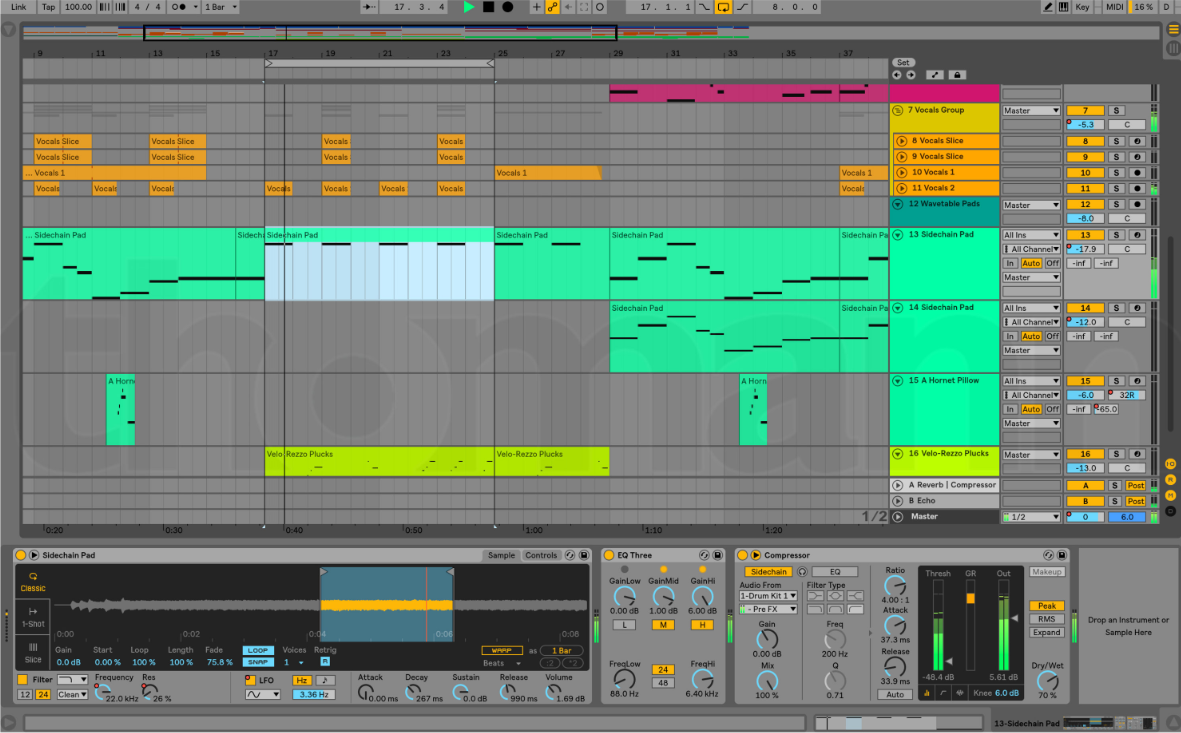
\includegraphics[scale=0.4]{./pictures/ableton.png}
\caption{Screenshot of Ableton Live GUI environment. Source: https://www.thomann.de/dk/ableton\_live\_10\_intro.htm}
\label{fig:ableton.png}
\end{figure}

\subsubsection{QLab}
QLab is a free download that combines audio, video and lightning control in one package (http://figure53.com/qlab/). QLab controls playback of these element during a live perfomance. The operator triggers events such as light-, audio- and video-cue(s) in a cue list, which contain cues to trigger an event that the user edited. \newline

\textbf{Audio Playback:} QLab allows end-user or designer to align audio files in sequential order. Once inserted in cue list, end-user can manipulate by looping, change amplitude, volume, fades, etc. End-user need external audio interface to route the audio to mixing board. More on audio interface later. \\

\textbf{Video Playback:} End-user or designer can add video to cue list for synchronization and modification in real time. End-user need video card to route video to a screen. Speed of CPU and video card can affect quality of video playback. Does not support Windows PC - Mac OS-X only. \\

\textbf{Pricing:} QLab cost from 4.00 USD/day for a 24-hour license to 999.00 USD for a one-time license purchase with all the features. Free version has limited features.

\begin{figure}[H]
\centering
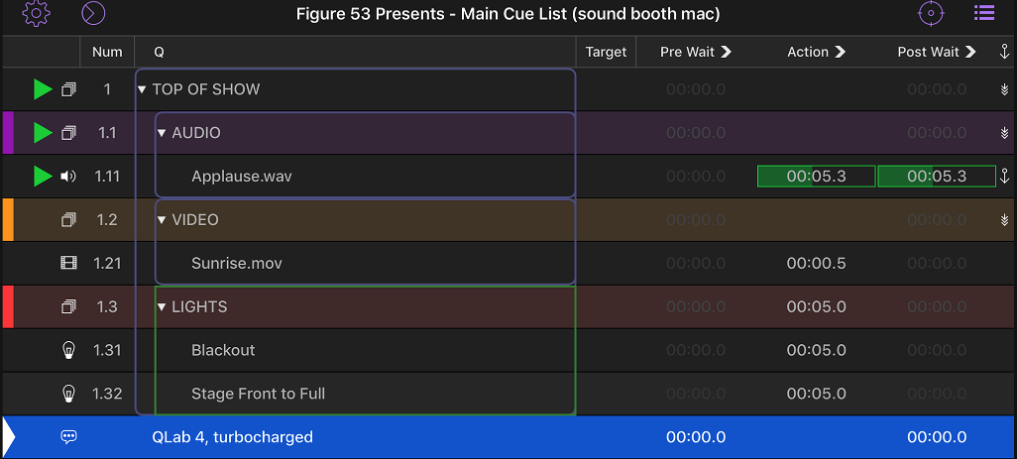
\includegraphics[scale=0.8]{./pictures/qlab.png}
\caption{Screenshot of QLab GUI environment. Source: (https://figure53.com/qlab/remote/)}
\label{fig:qlab.png}
\end{figure}

\subsubsection{Logic Pro X}
Logic Pro X is a DAW and MIDI sequencer software application for the Mac OS-X platform. Logic's primary function is music production, but is also widely used for playback in live performances. \newline

Developed by Apple Inc., the current proprietary license is released macOS. Logic version 5.5.1 wasthe last version bo be released for Windows. Version 6 and onward, Logic is only available for Mac OS. Like QLab, Logic need external audio interface to connect with mixing board. \\
 
\begin{figure}[H]
\centering
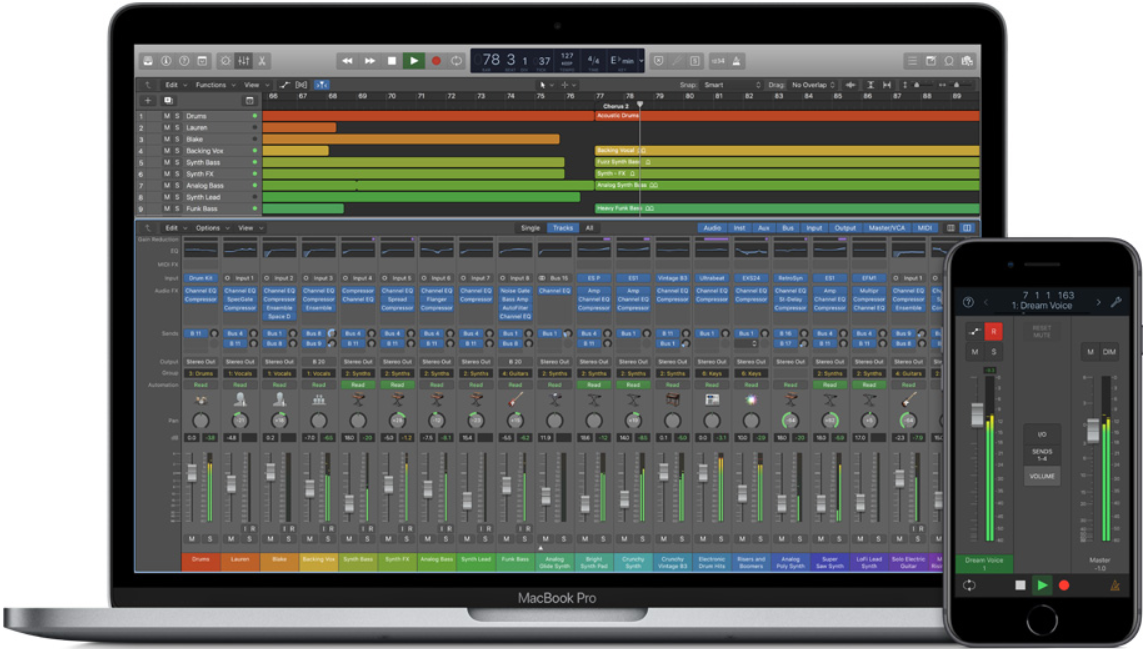
\includegraphics[scale=0.4]{./pictures/logic.png}
\caption{Screenshot of Logic software application. Source: https://www.apple.com/logic-pro/resources/}
\label{fig:logic.png}
\end{figure}

\textbf{Price:} 199.99 USD in App Store. \\

\subsubsection{MainStage}
Even though Apple's Logic Pro X is capable of playback of multichannel of audio, its primary function is music production: Recording and editing of audio tracks. \newline

MainStage is designed exclusively for live performances with a few key features, play back of pre-recorded backing tracks being the most notable feature. Like QLab and Logic, MainStage need external audio interface to connect with mixing board. \\
 
\begin{figure}[H]
\centering
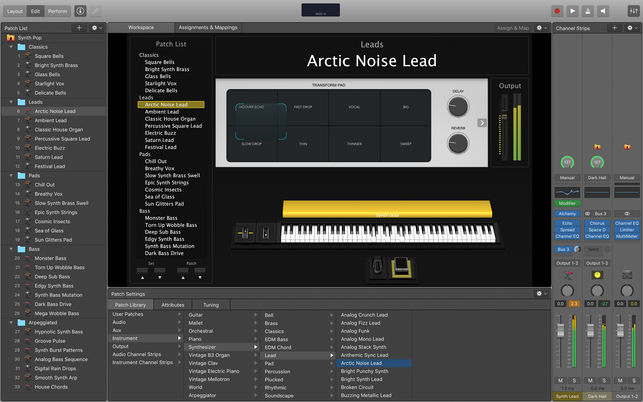
\includegraphics[scale=0.4]{./pictures/mainstage.png}
\caption{Screenshot of MainStage software application. Source: https://itunes.apple.com/dk/app/mainstage-3/}
\label{fig:mainstage.png}
\end{figure}

\textbf{Price:} 29.99 USD in App Store. \\

\subsubsection{Pro Tools}
Pro Tools is a DAW developed and release by Avid Technologies for Windows and masOS. Its many features include audio recording, music production, editing, post production, etc. \newline

Pro Tools can run as standalone software \textit{or} operate using external A/D converters, PCIe cards with onboard DSPs. Like QLab, Logic and MainStage, Pro Tools need external audio interface to connect with mixing board. \\

\begin{figure}[H]
\centering
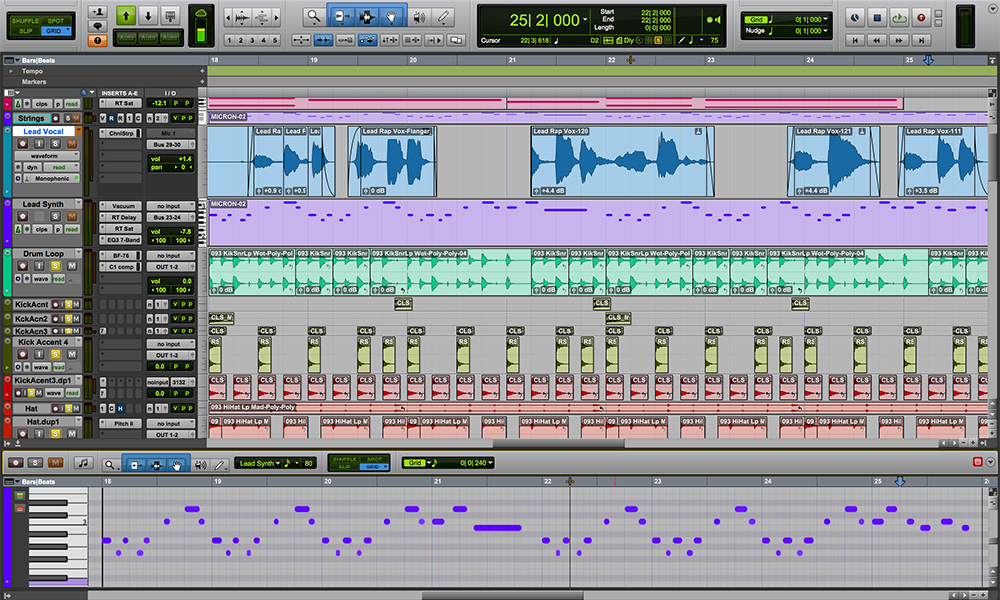
\includegraphics[scale=0.3]{./pictures/protools.png}
\caption{Screenshot of Pro Tools software application. Source: https://www.avid.com/pro-tools/features/}
\label{fig:protools.png}
\end{figure}

\textbf{Price:} From free software for Pro Tools | First with limited features to  559,00 EUR for one-time purchase with annual upgrade plan.

\subsubsection{Open Source Products}
Quite a few Do-It-Yourself (DIY) builders, enthusiasts, hobbyists and likeminded individuals have attempted to produce similar products with various degrees of success. \newline

Several open source technologies are available for product development:\textbf{Arduino} (https://www.arduino.cc/), \textbf{Raspberry Pi} (https://www.raspberrypi.org/) and \textbf{BeagleBone Black} (https://beagleboard.org/black) counts as the most widely used technologies. \newline

As Showman is intended for market release for consumers and prosumers, open source solutions are not within the scope of the project at the moment as additional research in open source regulations and their marketability is necessary - A research that can lead the project to a sidetrack and the time frame does not allow for in-depth investigations. \\

\subsubsection{Showman}
The intended features for Showman is shown in Figure ~\ref{fig:showman.png}

\begin{figure}[H]
\centering
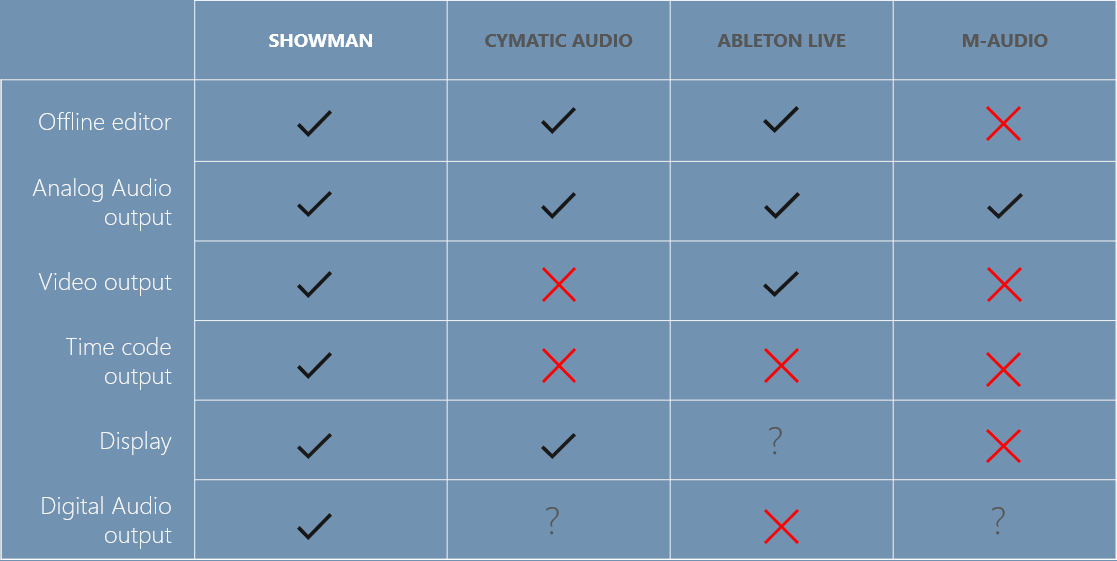
\includegraphics[scale=0.5]{./pictures/showman.png}
\caption{Intended features for Showman with a comparison matrix of competing producers.}
\label{fig:showman.png}
\end{figure}

\subsection{Literature}
As mentioned in the description, a research in these subjects are needed for design, implementation and test of Showman: \\

For design and implementation of the device, a research is needed in: \\
- Circuit/hardware design \\
- D/A audio converters \\
- Standardized audio input/output formats \\
- Audio file formats \\
- Standardized video input/output formats \\
- Video file formats \\
- Time codes for synchronization \\
- User feedback for feasible GUI design \\

Selected chapters from: \\
\textbf{Ken C. Pohlmann}: Principles of Digital Audio Sixth Edition. (\textbf{ISBN: 987-0-07-166346-5}). This is the starting point for the literature. Additional textbooks from the AU Library or from other sources will be investigated when additional information becomes relevant. \\

\textbf{Eddy Bøgh Brixen}: Praktisk Elektroakustik 3. udgave. \textbf{ISBN: 9788791117206}. This textbook introduces several audio concepts necessary for Showman's features such as XLR-plugs, file formats, etc. \\ 

\textbf{User Manuals}: User manuals from competing producers are necesary to understand the design process. Some of these contain block diagrams that can be useful for Showman when modified to suit Showman's needs. \\

\textbf{Datasheets}: In addition to textbooks, datasheets for relevant parts will be investigated thoroughly and evaluated upon before implementation. \\

\textbf{GUI Design}: Research in GUI design is a must have for design of software application GUI. It was the project's wish to work as a team with a more experienced programmer and student from the \textbf{Information and Communication Technology} branch of ASE, but none were available. However, 2 programmers has expressed interest in occassional assistance and guidance during design and implementation process of GUI.
\chapter{Project Expectations}
\textbf{Showman and SEMI Sound - Background} \\
SEMI Sound is a startup founded by \textbf{Se}bastian Wolff and \textbf{Mi}nik Nathanielsen Olsen to develop and produce technologies for touring artists. Both Sebastian and Minik have many years of touring experience  as musician and sound engineer respectively. The concept for Showman was born around 2013-2014 after a series of performances with Sebastian's band (who employs Minik as backliner and monitor audio engineer), when the performances suffered technical difficulties caused by a malfunctioning hard disk recorder used for playback of backing tracks. \newline

Preparation for a tour is commonly referred to as \textit{pre-production}. During pre-production for a Summer tour in 2018, the band abandoned the idea of re-using the hard disk recorder in favor of the LP-16 Live Player as a temporary solution; Showman's additional features are needed for the next tour cycle. This motivated Minik to develop the Showman concept further and use the band as betatesters. Inspired by this, Minik decided to develop Showman as NSI Startup Factory as part of his apprenticeship period before continuing the project as part of the Bachelor's Project. To avoid a 6-month gap, Minik swapped 5th and 6th semester in order to work full-time on the project without interruptions. \newline

\section{Workplace}
\textbf{Workplace} \\
After initial project proposal was accepted, an application for project working space was filed to secure an assigned working space at the university campus. As of this document's handin, no working space has been assigned yet as deadline for application handin is January 11th. \\

Meeting with supervisor before initiating work on this document, it was announced that the project will be supervised jointly with 2 other projects who also work independently. Supervisor proposes that the 3 project share workplace to encourage a better work ethic which can be elusive on solo projects. \\

\textbf{Lab work} \\
Additionally, access to ASE's lab is crucial for the project when implementing and testing design. \\

\textbf{Working from home} \\
Living in Esbjerg, some 180 kilometers from ASE, it is expected to do some work at home as well. However, primary workplace during the weekdays is at ASE. \\

\section{Platform}
Initially, the \textbf{HDMI Audio EI3 EZ-Extender} (https://www.analog.com/en/design-center/evaluation-hardware-and-software/evaluation-boards-kits/eI3-hdmiaudio.html\#eb-overview) evaluation board was chosen as platform for Showman prototype. But it is not available at the moment, but \textit{used} boards are available online. \\

\begin{figure}[H]
\centering
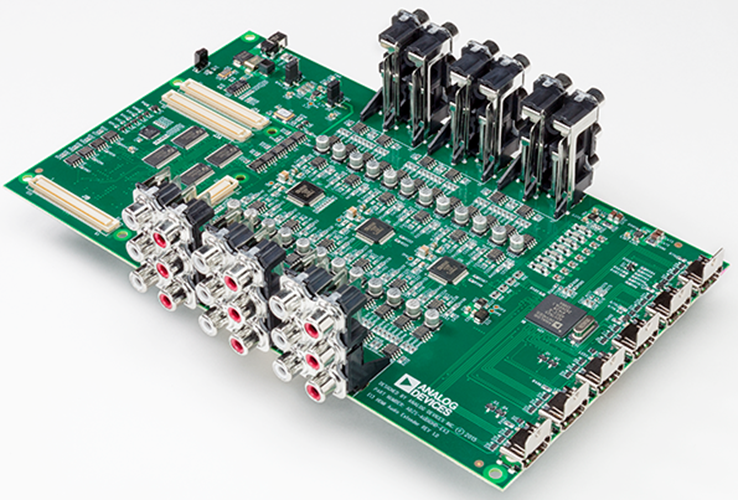
\includegraphics[scale=1]{./pictures/ei3.png}
\caption{Initial platform for development: \textbf{HDMI Audio EI3 EZ-Extender}. Rejected as it is currently unavailable from the vendor.}
\label{fig:ei3.png}
\end{figure}

For the audio part of Showman, \textbf{EVAL-21469-EZLITE} (https://www.analog.com/en/design-center/evaluation-hardware-and-software/evaluation-boards-kits/21469-ezlite.html\#eb-overview) is now the chosen platform. \\

\begin{figure}[H]
\centering
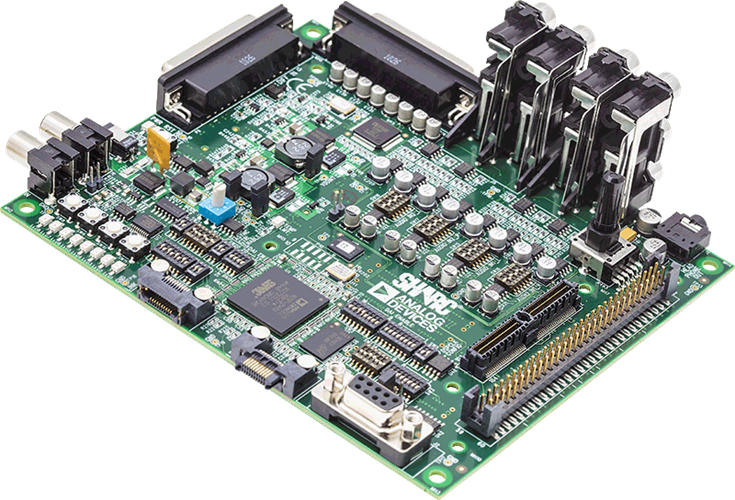
\includegraphics[scale=0.4]{./pictures/ADZS.png}
\caption{Requested platform for development: \textbf{EVAL-21469-EZLITE}.}
\label{fig:ADZS.png}
\end{figure}

\textbf{Price:} 574.20 USD + shipping \\ 

Research on video part is ongoing at the moment.

\section{Project Funding}
\subsection{Foundations}
As the price for the ADSP-2146x EZ-KIT Lite exceeds the maximum for university expense coverage, project funding from the university is not available. The necessary project funding need to be covered by external funds from initiatives such as InnoFounder, InnoBooster, etc. Applications for funding is currently in the works and essential material needed before the project begins is currently covered by Minik. \\

\subsection{Grants}
Concurrently with funding applications, applications for grants and donations are also in the works. \\

\subsection{Private Funding}
If applications from foundations and grants are refused, necessary funding will be covered by private funds from own savings. \\

\section{Beta Testers}
Having a large network of musicians, sound engineers and other touring personnel, a 2 other bands have been recruited as betatesters when the project is ready to test Showman. \newline

\chapter{Conclusion}
Konklusion på det indledende arbejde med forprojektet.
%include content sections here
%\input{briefUseCases}
%input{SPI_Devkit_PSoC_doc.tex}
\backmatter

%appendix, biblography, index, list of tables, list of figures should be placed here.
\listoffigures

%\listoftables

%\newpage
%\printbibliography
\end{document}